\def\PicPath{/Users/ken/Documents/shuron/chapter1}
\chapter{MeVガンマ線天文学}
\begin{comment}
%天文学は色々な波長のよる観測で進んできた
天文学は可視光から電波・赤外線・X線と様々な波長の電磁波の観測を行うことで発展してきた。さらに今日では陽子を主とする宇宙線やニュートリノなどの観測も行われる様になり、観測によって得ることが可能な宇宙の情報はより豊かになった。

%ガンマ線天体観測と色々な波長について
宇宙の情報を得る手段の一つとしてガンマ線観測が挙げられる。ガンマ線とは数百keV以上のエネルギーを持つ電磁波を指す。1950年代に早川らにより、宇宙線と星間物質との相互作用で作られる$\pi^{0}$中間子の崩壊によってガンマ線が放射されることが予言されて以来1967年にOSO-3($\geq$ 50$\ $kev)、1972年にSAS-2(20\ MeV $\sim$ 1$\ $GeV)、1975年にCOS-B(2 $\ $keV $\sim$ 5$\ $GeV)と、次々とガンマ線観測衛星が打ち上げられ、多くのガンマ線天体を発見している。また、sub-MeV$\sim$数十MeVまでの低エネルギーガンマ線では、1989年にGRANT衛星がロシア、フランスによって、1991年にCGRO衛星がアメリカによって打ち上げられている。近年は20022年に硬X線を観測するINTEGRAL、2004年にガンマ線バーストを観測するSWIFT、2008年にGeV領域を観測するFermiが打ち上げられ、観測を続けている。地上では1990年代からWhipple、CANGAROOなどのCherenkov望遠鏡によって非常にエネルギーの高いTeVガンマ線領域の観測が始まっており、現在でもステレオ方式のHESS、MAGIC等によって次々と新しいガンマ線天体が発見されている。

%MeVガンマ線を観測すると色々なことが解明されると期待されている
MeV領域のガンマ線は元素合成や粒子加速、宇宙線と星間物質との相互作用といった情報を提供する。また、MeVガンマ線は高エネルギーガンマ線とは異なり、最遠方の初期宇宙から地球までほとんど減衰することはない。そのため、初期宇宙の激しい星の生成、消滅などの観測が期待されるユニークなガンマ線である。しかし、一方で地球の大気には吸収されるため、MeVガンマ線の観測は大気外に出る必要がある。(図\ref{fig:atm_absp})
\begin{figure}
\centering
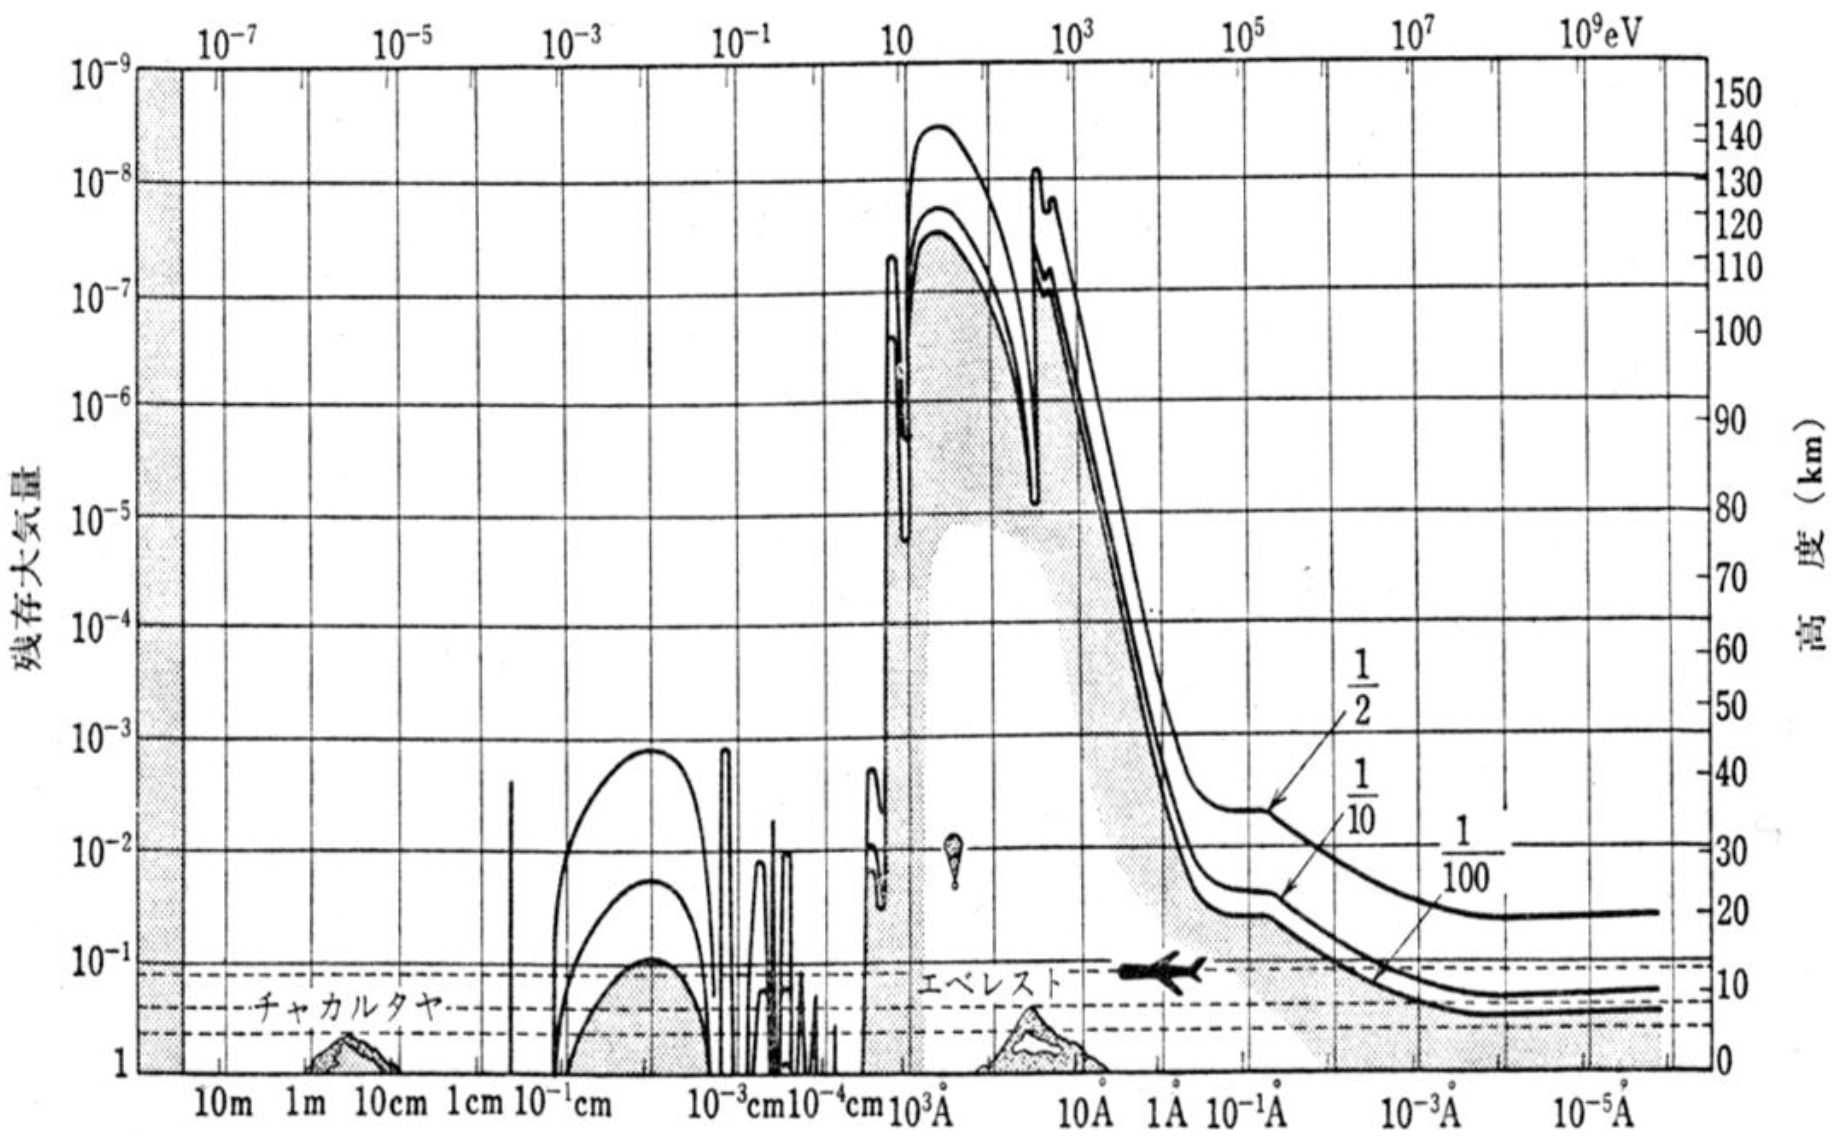
\includegraphics[width=15cm]{\PicPath/atmosphere_absorption.png}
\caption{大気による様々な波長の電磁波の吸収\cite{oda_and_matsuoka}}
\label{fig:atm_absp}
\end{figure}

%MeVガンマ線の観測には様々な困難を伴うため、あまり進んでいない
MeV領域は可視光やX線の領域に比べ、光子数が少なく透過力も高い上、物質との相互作用が主にコンプトン散乱によるので光子の完全な吸収は難しい。さらに銀河面全体に広がったガンマ線放射や、宇宙線と衛星本体との相互作用による大量のバックグラウンドが存在し、観測が非常に困難な領域である。以上の理由から、MeV領域の天文学は、他の波長域に比べ大きく遅れを取っているのが現状である。

この章ではMeVガンマ線領域について簡単に解説し、これまで行われてきたMeVガンマ線観測、そしてMeVガンマ線を観測することでどの様な物理現象の解明に繋がると期待されているかについて述べる。
\end{comment}

%
%天文学は色々なものを観測することで発展してきた
宇宙の観測は地上から可視光を観測することから始まり、現在では人工衛星を用いることで宇宙空間において可視光は勿論、電波・赤外線・X線の領域の観測が行われるまでになり、電磁波以外にも陽子を主とする宇宙線やニュートリノの観測なども行われるようになった。このように様々な側面から宇宙を観測することで天体の多種多様で興味深い振る舞いが数多く明らかになっていき、天文学は今日まで発展し続けてきた。

%中でもMeVガンマ線というものは、観測することで〜〜といった物理現象の解明が期待されている
中でもMeVガンマ線という側面からは放射性同位体が崩壊する時に放射される数百keV$\sim$数MeVの核ガンマ線を観測できるので元素合成の過程の解明に繋がると期待されている。
%実際にMeVガンマ線を観測するためにCOMPTELだとかが上がったけどそんなに大きな成果は出していない(不十分)
しかし、MeVガンマ線はその性質から観測が困難であり、現在までに十分な感度による観測は行われておらず未開拓な部分が多い領域でもある。
この章では、まずMeVガンマ線領域の性質について簡単に述べてから、MeVガンマ線を観測することで解明が期待されているいくつかの物理事象を現在までの観測結果と共に述べていく。

\section{これまでのMeVガンマ線天文学}
\subsection{MeVガンマ線領域}

画像だよ画像だよ画像だよ画像だよ画像だよ画像だよ画像だよ画像だよ画像だよ画像だよ画像だよ画像だよ画像だよ画像だよ画像だよ画像だよ画像だよ画像だよ画像だよ画像だよ画像だよ画像だよ画像だよ画像だよ画像だよ画像だよ画像だよ画像だよ画像だよ画像だよ画像だよ画像だよ画像だよ画像だよ画像だよ画像だよ画像だよ画像だよ画像だよ画像だよ画像だよ画像だよ画像だよ画像だよ画像だよ画像だよ画像だよ画像だよ画像だよ画像だよ画像だよ画像だよ画像だよ画像だよ画像だよ画像だよ画像だよ画像だよ画像だよ画像だよ画像だよ画像だよ画像だよ画像だよ画像だよ画像だよ画像だよ画像だよ画像だよ画像だよ画像だよ画像だよ画像だよ画像だよ画像だよ画像だよ画像だよ画像だよ画像だよ画像だよ画像だよ画像だよ画像だよ画像だよ画像だよ画像だよ画像だよ
\begin{figure}
\centering
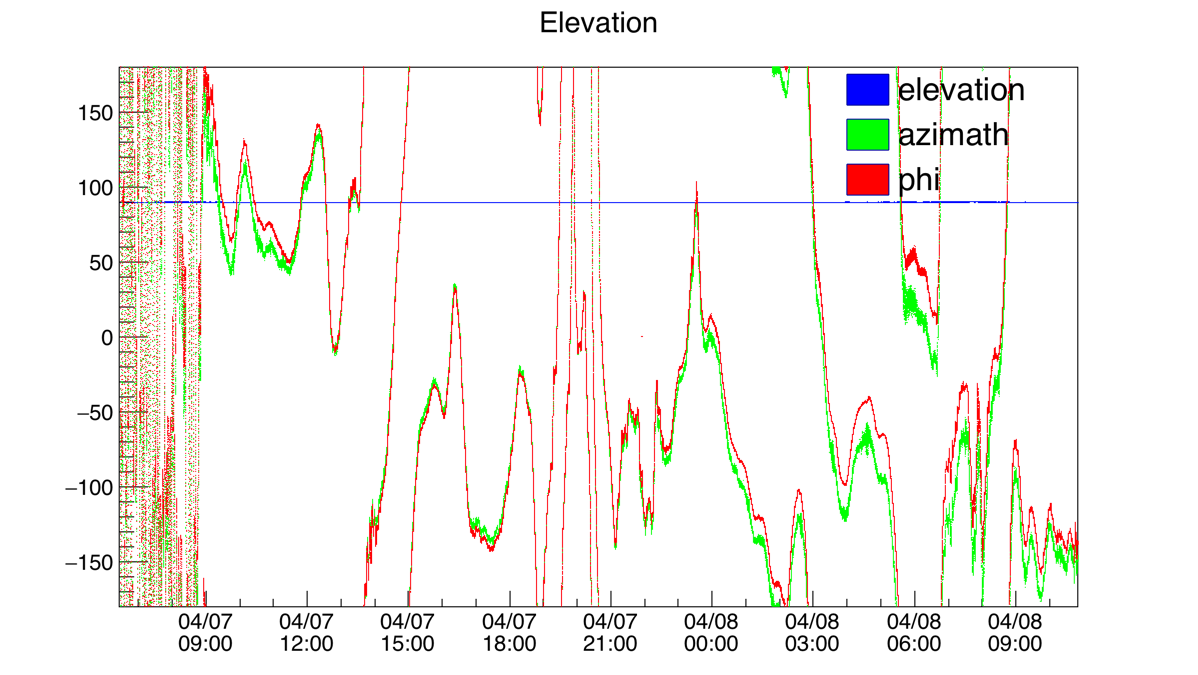
\includegraphics[width=15cm]{attitude_f.png}
\caption{test}
\end{figure}

\def\PicPath{/Users/ken/Documents/shuron/chapter1/1_2}

\begin{comment}

(図\ref{fig:science_sensitivity})
\begin{figure}
\centering
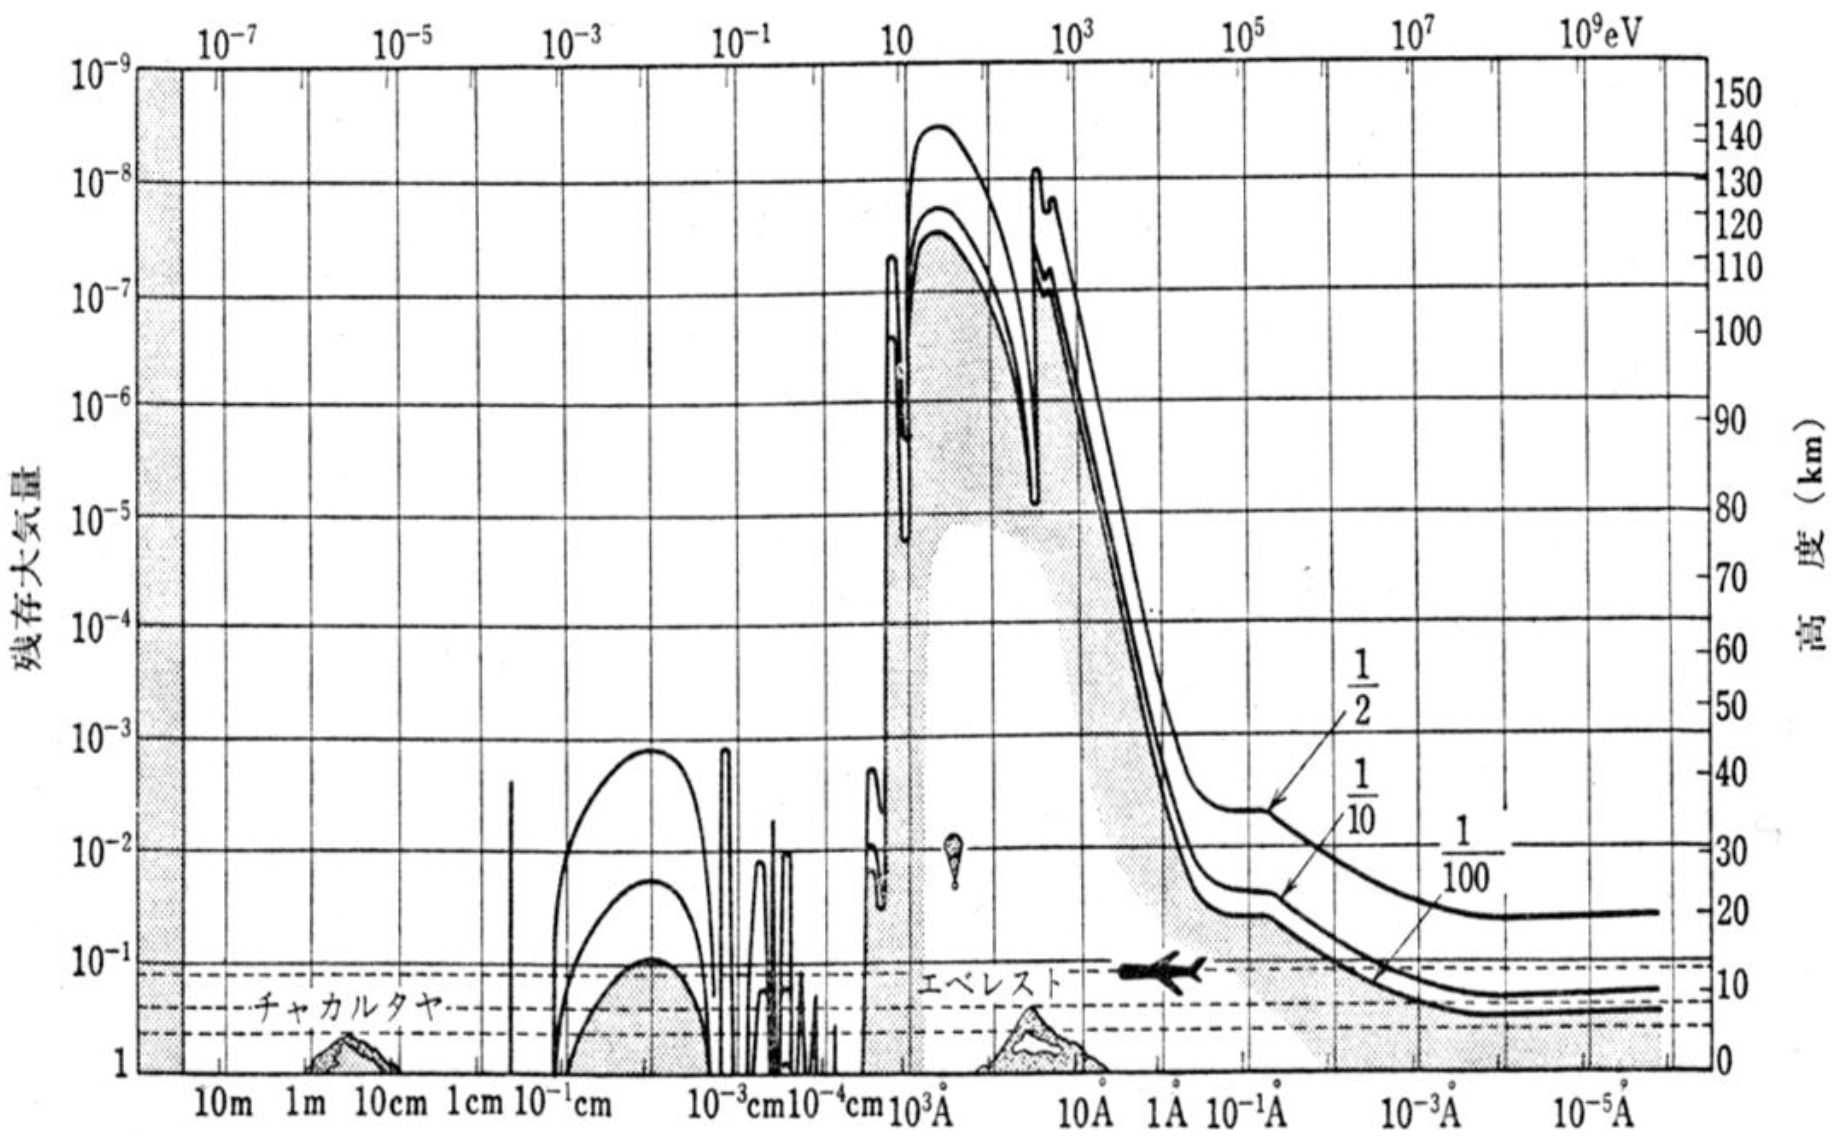
\includegraphics[width=15cm]{\PicPath/atmosphere_absorption.png}
\caption{大気による様々な波長の電磁波の吸収(出典??)\cite{oda_and_matsuoka}}
\label{fig:atm_absp}
\end{figure}

\end{comment}

\section{核ガンマ線観測}
核ガンマ線の観測をするとめっちゃうれしいよ!こういうことがわかるしなんでもわかる
\subsection{核ガンマ線}
てすとてすと
\subsection{Ia}
テストテスト
\subsection{重力崩壊型}
テストテスト




